% Customizable fields and text areas start with % >> below.
% Lines starting with the comment character (%) are normally removed before release outside the collaboration, but not those comments ending lines

% svn info. These are modified by svn at checkout time.
% The last version of these macros found before the maketitle will be the one on the front page,
% so only the main file is tracked.
% Do not edit by hand!
\RCS$Revision: 92718 $
\RCS$HeadURL: svn+ssh://alverson@svn.cern.ch/reps/tdr2/notes/RutgersMCGuide/trunk/RutgersMCGuide.tex $
\RCS$Id: RutgersMCGuide.tex 92718 2011-12-22 22:37:09Z alverson $

%%%%%%%%%%%%% local definitions %%%%%%%%%%%%%%%%%%%%%
% This allows for switching between one column and two column (cms@external) layouts
% The widths should  be modified for your particular figures. You'll need additional copies if you have more than one standard figure size.
\newlength\cmsFigWidth
\ifthenelse{\boolean{cms@external}}{\setlength\cmsFigWidth{0.85\columnwidth}}{\setlength\cmsFigWidth{0.4\textwidth}}
\ifthenelse{\boolean{cms@external}}{\providecommand{\cmsLeft}{top}}{\providecommand{\cmsLeft}{left}}
\ifthenelse{\boolean{cms@external}}{\providecommand{\cmsRight}{bottom}}{\providecommand{\cmsRight}{right}}

% A rudimentary config that shows off some features.
%\lstset {
%basicstyle=\ttfamily\scriptsize, % Without beramono, we'd get cmtt, the teletype font.
%commentstyle=\textit\scriptsize, % cmtt doesn't do italics. It might do slanted text though.
%breaklines=true
%}

% --- force emacs to latex mode -*-latex-*-
%
% Tell TeX where to look for graphics files to be included
%
\graphicspath{{pdf/}} % Note, the additional {} are mandatory!
\renewcommand\topfraction{.95}
\renewcommand\bottomfraction{.95}
\renewcommand{\floatpagefraction}{0.9}
\renewcommand{\textfraction}{0.05}
\topmargin 0mm
\oddsidemargin 0mm
\textwidth 170mm
\textheight 230mm
%
% Put additional commands, abbreviations etc. here
%
\newcommand{\jt}{\ensuremath{H_{\mathrm{T}}}\xspace}
\newcommand{\GeVC}{\ensuremath{\GeV\!/c}}
\newcommand{\gevc}{\ensuremath{\GeV\!/c}}
\newcommand {\abseta} {|\eta|}
\newcommand{\mzero}{\ensuremath{{m_0}}}
\newcommand{\azero}{\ensuremath{A_{0}}}
\newcommand{\mhalf}{\ensuremath{m_{1/2}}}
\newcommand{\tb}{\ensuremath{\tan\beta}}

% Sleptons
\providecommand{\slepton}{\ensuremath{\widetilde{\ell}}\xspace}
\providecommand{\selectron}{\ensuremath{\widetilde{\cmsSymbolFace{e}}}\xspace}
\providecommand{\smuon}{\ensuremath{\widetilde{\mu}}\xspace}
\providecommand{\stau}{\ensuremath{\widetilde{\tau}}\xspace}

% Squarks
\providecommand{\squark}{\ensuremath{\widetilde{\cmsSymbolFace{q}}}\xspace}
\renewcommand{\sbone}{\ensuremath{\widetilde{\cmsSymbolFace{b}}_{1}}\xspace}
\renewcommand{\stop}{\ensuremath{\widetilde{\cmsSymbolFace{t}}}\xspace}

% Neutralinos
\providecommand{\nall}{\ensuremath{\widetilde{\chi}^{0}}\xspace}
\providecommand{\nalli}{\ensuremath{\widetilde{\chi}^{0}_{i}}\xspace}
\providecommand{\none}{\ensuremath{\widetilde{\chi}^{0}_{1}}\xspace}
\providecommand{\ntwo}{\ensuremath{\widetilde{\chi}^{0}_{2}}\xspace}
\providecommand{\nthree}{\ensuremath{\widetilde{\chi}^{0}_{3}}\xspace}

% Charginos
\providecommand{\call}{\ensuremath{\widetilde{\chi}^{\pm}}\xspace}
\providecommand{\cone}{\ensuremath{\widetilde{\chi}^{\pm}_{1}}\xspace}
\providecommand{\conem}{\ensuremath{\widetilde{\chi}^{-}_{1}}\xspace}
\providecommand{\conep}{\ensuremath{\widetilde{\chi}^{+}_{1}}\xspace}
\providecommand{\ctwo}{\ensuremath{\widetilde{\chi}^{\pm}_{2}}\xspace}

% Gluinos
\providecommand{\gluino}{\ensuremath{\widetilde{g}}\xspace}

% Gravitino or Goldstino
\providecommand{\goldstino}{\ensuremath{\widetilde{\cmsSymbolFace{G}}}\xspace}

\newcommand{\nunit}[2]{#1\,\mbox{#2}}
\newcommand{\met}{\ensuremath{E_{\mathrm{T}}^{\text{miss}}}\xspace}
\newcommand{\curlumi}{714}
\providecommand{\FIXME}[1]{({\bf FIXME: #1})}
\providecommand{\HERWIGPP} {{\textsc{herwig++}}\xspace}
\providecommand{\JIMMY} {{\textsc{jimmy}}\xspace}
\providecommand{\NLOJETPP} {{\textsc{nlojet++}}\xspace}
\providecommand{\Et}{E_{\mathrm{T}}}
%\providecommand{\met}{\mbox{${\hbox{$\vec{E}$\kern-0.5em\lower-.1ex\hbox{/}}}_T~$}}
%\providecommand{\MET}{\mbox{${\hbox{$E$\kern-0.5em\lower-.1ex\hbox{/}}}_T~$}}
\providecommand{\pthat}{\ensuremath{\hat{\text{p}}_\mathrm{T}}\xspace}
\providecommand{\kthat}{\ensuremath{\hat{\text{k}}_\mathrm{T}}\xspace}
\providecommand{\xt}{\ensuremath{\text{x}_\mathrm{T}}\xspace}
\providecommand{\ptjet}{\ensuremath{p_{\mathrm{T,jet}}}\xspace}
\providecommand{\FASTNLO} {{fast\textsc{nlo}}\xspace}

\providecommand{\rbthm}{\rule[-2ex]{0ex}{5ex}}
\providecommand{\rbthr}{\rule[-1.7ex]{0ex}{5ex}}
\providecommand{\rbtrm}{\rule[-2ex]{0ex}{5ex}}
\providecommand{\rbtrr}{\rule[-0.8ex]{0ex}{3.2ex}}
\providecommand{\relmet}{\ensuremath{\text{MET}/\sum{E_{\mathrm{T}}}}}
\providecommand{\LvStartup}{\ensuremath{\mathcal{L}=\text{10}^\text{31}\,\text{cm}^\text{$-$2}\,\text{s}^\text{$-$1}}\xspace}

% \newcommand{\ptof}[1]{p_{\mathrm{T}}^{\mathrm{#1}}}
% \newcommand{\ptcalo}{\ptof{calo}}
% \newcommand{\ptgen}{\ptof{gen}}
% \newcommand{\ptz}{\ptof{Z}}
% \newcommand{\ptcontrol}{\ptof{control}}
% \newcommand{\ltwodijet}{L2$^{\mathrm{MC dijet}}$\ }
% \newcommand{\lthreedijet}{L3$^{\mathrm{MC dijet}}$\ }
% \newcommand{\Kt}{K$_{\mathrm{T}}$}
% \newcommand{\Eti}{E_{\mathrm{T}}^i}

% Already defined in ptdr-definitions
%\newcommand{\fixme}[1]{
%  \mbox{} \\
%  XXXXXXXXXX START XXXXXXXXXXXXX \\
%  {#1} \mbox{} \\
%  XXXXXXXXXXX END XXXXXXXXXXXXX \\
%}
%\newcommand{\pt}{p_{\mathrm{T}}}
%\newcommand{\kt}{k$_{\mathrm{T}}$}
\newcommand{\procLumi}{19.5~\textrm{fb}^{-1}}
%\newcommand{\ttbar}{\ensuremath{{t\overline{t}}}\xspace}
\newcommand{\iso}{\mathrm{iso}}
\newcommand{\noniso}{\mathrm{noniso}}
\newcommand{\eiso}{\epsilon_\iso}
\newcommand{\eisomu}{\eiso(\mu)}
\newcommand{\eisotr}{\eiso(\mathrm{track})}
\newcommand{\esb}{\epsilon_\mathrm{sb}}
%\newcommand{\Pp}{\ensuremath{\mathrm{p}}}
%\newcommand{\Pgm}{\ensuremath{{\mu}}}
%\newcommand{\Pem}{\ensuremath{\mathrm{e}^-}}
%\newcommand{\Pep}{\ensuremath{\mathrm{e}^+}}
%\newcommand{\Pe}{\ensuremath{\mathrm{e}}}
%\newcommand{\PJgy}{\ensuremath{\mathrm{J}\hspace{-.08em}/\hspace{-.14em}\psi\mathrm{(1S)}}}
%\newcommand{\PgU}{\ensuremath{\Upsilon}}
%\newcommand{\PgUa}{\ensuremath{\Upsilon\mathrm{(1S)}}}
%\newcommand{\PgUb}{\ensuremath{\Upsilon\mathrm{(2S)}}}
%\newcommand{\PgUc}{\ensuremath{\Upsilon\mathrm{(3S)}}}
%\newcommand{\PgUd}{\ensuremath{\Upsilon\mathrm{(3S)}}}
%\newcommand{\PgUe}{\ensuremath{\Upsilon\mathrm{(10860)}}}
%\newcommand{\PgUf}{\ensuremath{\Upsilon\mathrm{(11020)}}}
%\newcommand{\GeV}{\mbox{GeV}\xspace}
%\newcommand{\pt}{\ensuremath{p_{\mathrm{T}}}\xspace}
%\newcommand{\et}{\ensuremath{E_{\mathrm{T}}}\xspace}
%\newcommand{\GeVc}{\mbox{GeV/$c$}\xspace}
%\newcommand{\GeVcc}{\mbox{GeV/$c^2$}\xspace}

%Definitions from TWIKI note
\def\beq{\begin{equation}}
\def\eq{\end{equation}}
\def\eeq{\end{equation}}

\def\fivelep{\ell \ell \ell \ell \ell}
\def\fourlep{\ell \ell \ell \ell} 
\def\threelep{\ell \ell \ell} 
\def\twolep{\ell \ell} 


%\def\beq{\begin{equation}}
\def\eq{\end{equation}}
%\def\eeq{\end{equation}}
\def\bea{\begin{eqnarray}}
\def\eea{\end{eqnarray}}

%\def\l{l}
\def\l{\ell}

\def\chii0{\chi_i^0}
\def\chij0{\chi_j^0}
\def\chiipm{\chi_i^{\pm}}
\def\chijpm{\chi_j^{\pm}}
\def\chiimp{\chi_i^{\mp}}
\def\chijmp{\chi_j^{\mp}}

%\def\none{\chi_1^0}
%\def\cone{\chi_1^{\pm}}


\def\ETslash{\not \! \! E_T}

% fromto command for rightangle to rightarrow

\def\fromto{ \put(4,2.85){\line(0,1){12}} \to }
\def\longfromto{ \put(4.45,2.85){\line(0,1){12}} \longrightarrow }


%%%%%%%%%%%%%%%  Title page %%%%%%%%%%%%%%%%%%%%%%%%
\cmsNoteHeader{RutgersMCGeneration} % This is over-written in the CMS environment: useful as preprint no. for export versions
% >> Title: please make sure that the non-TeX equivalent is in PDFTitle below
\title{A Guide to Monte Carlo Production}

% >> Authors
%Author is always "The CMS Collaboration" for PAS and papers, so author, etc, below will be ignored in those cases
%For multiple affiliations, create an address entry for the combination
\address[rutgers]{Rutgers University}
\author[rutgers]{C. Contreras-Campana, E. Contreras-Campana, P. Thomassen, M. Walker, P. Zywicki}

% >> Date
% The date is in yyyy/mm/dd format. Today has been
% redefined to match, but if the date needs to be fixed, please write it in this fashion.
% For papers and PAS, \today is taken as the date the head file (this one) was last modified according to svn: see the RCS Id string above.
% For the final version it is best to "touch" the head file to make sure it has the latest date.
\date{\today}

% >> Abstract
% Abstract processing:
% 1. **DO NOT use \include or \input** to include the abstract: our abstract extractor will not search through other files than this one.
% 2. **DO NOT use %**                  to comment out sections of the abstract: the extractor will still grab those lines (and they won't be comments any longer!).
% 3. **DO NOT use tex macros**         in the abstract: External TeX parsers used on the abstract don't understand them.
\abstract{The purpose of this note is to document the accumulated knowledge that 
Rutgers has acquired over the years for the production of Monte Carlo (MC) events. 
We will cover ISAJET, which generate SLHA files, leading-order (LO) MC event 
generators like $\PYTHIA$ and $\MADGRAPH$, validation tools, the CMS software 
(CMSSW), $\PROSPINO$2, which is a next-to-leading order (NLO) cross section 
calculator, and the recommended program for producing Feynman diagrams.}

% >> PDF Metadata
% Do not comment out the following hypersetup lines (metadata). They will disappear in NODRAFT mode and are needed by CDS.
% Also: make sure that the values of the metadata items are sensible and are in plain text (no TeX! -- for \sqrt{s} use sqrt(s) -- this will show with extra quote marks in the draft version but is okay).

\hypersetup{%
pdfauthor={C. Contreras-Campana, E. Contreras-Campana, P. Thomassen, M. Walker, P. Zywicki},%
pdftitle={CMS Paper Template 2006 LaTeX/PdfLaTeX version},%
pdfsubject={CMS},%
pdfkeywords={CMS, physics, software, computing, MC production}}

\maketitle %maketitle comes after all the front information has been supplied
% >> Text
%%%%%%%%%%%%%%%%%%%%%%%%%%%%%%%%  Begin text %%%%%%%%%%%%%%%%%%%%%%%%%%%%%
%% **DO NOT REMOVE THE BIBLIOGRAPHY** which is located before the appendix.
%% You can take the text between here and the bibiliography as an example which you should replace with the actual text of your document.
%% If you include other TeX files, be sure to use "\input{filename}" rather than "\input filename".
%% The latter works for you, but our parser looks for the braces and will break when uploading the document.
%%%%%%%%%%%%%%%
\tableofcontents
\newpage

%\listoffigures
%\newpage

%\listoftables
%\newpage

%%%%%%%%%%%%% Overview %%%%%%%%%%%%%%%%%%%%%
\section{Overview}

%%%%%%%%%%%%% ISAJET %%%%%%%%%%%%%%%%%%%%%
\section{\texorpdfstring{$\ISAJET$}{ISAJET}}
\subsection{Introduction}

$\ISAJET$ 7.83  is a Monte Carlo program which simulates $\Pp \Pp$, $\Pp \bar{\Pp}$, and $\EE$ 
interactions at high energies~\cite{Baer:1999sp}. It is based on perturbative QCD plus phenomenological 
models for parton and beam jet fragmentation. The manual describes the physics and explains 
how to use the program.

$\ISAJET$ is written in FORTRAN 77 (with a few common extensions) and is distributed using the 
Patchy code management system developed at CERN. The Patchy source file isajet.car can be be 
unpacked and compiled on any supported Unix system by editing the Makefile and selecting the 
appropriate options. Compiling $\ISAJET$ on any other computer with ANSI Fortran 77 and Patchy, 
including any for which CERNlib is supported, should be straightforward.

This should produce the following executables: isajet.x, isasusy.x and isasugra.x. 
You can run make clean to get rid of the temporary files.

\subsection{Producing SLHA files with \texorpdfstring{$\ISAJET$}{ISAJET}}

No information about $\ISAJET$ will be included at this time.

\subsection{Producing SLHA files with \texorpdfstring{$\ISASUSY$}{ISASUSY}}

We give here an example of how to run $\ISASUSY$ interactively.
\small
\begin{verbatim}
[shell prompt]$ ./isasusy.x 
 ENTER output file name (in single quotes)
'HadronicRPV_squark1000_gluino1000.dat' <enter>
 ENTER SUSY Les Houches Accord filename [/ for none]:
HadronicRPV_squark1000_gluino1000_temp.slha <enter>
 ENTER Isawig (Herwig interface) filename [/ for none]:
HadronicRPV_squark1000_gluino1000.hwg <enter>
 ENTER M(TP)
172 <enter>
 ENTER M(GLSS), MU, M(A), TAN(BETA)
1000,3000,4000,3 <enter>
 ENTER M(Q1), M(DR), M(UR), M(L1), M(ER)
5000,1000,1000,4000,300 <enter>
 ENTER M(Q3), M(BR), M(TR), M(L3), M(LR), A_T, A_B, A_L
5000,1000,1000,4000,300,1000,9000,9000 <enter>
 ENTER OPTIONAL 2ND GEN MASSES (/ FOR DEFAULT):
 ENTER M(Q2), M(SR), M(CR), M(L2), M(MR)
/ <enter>
 ENTER OPTIONAL GAUGINO MASSES M1, M2 (/ FOR DEFAULT):
500,150 <enter>
 ENTER OPTIONAL GRAVITINO MASS (/ FOR DEFAULT):
/ <enter>
\end{verbatim}
\normalsize

The SLHA file has to be corrected with using an awk script.
\small
\begin{verbatim}
[shell prompt]$ awk -f SLHAprocessing.awk 
HadronicRPV_squark1000_gluino1000_temp.slha 
> HadronicRPV_squark1000_gluino1000.slha
[shell prompt]$ rm HadronicRPV_squark1000_gluino1000_temp.slha
\end{verbatim}
\normalsize

We have included an example in the appendix on how to run $\ISASUSY$ in a 
shell script (See Listing~\ref{lst:HadronicRPV}). The shell script runs with the following command, 
\small
\begin{verbatim}
[shell prompt]$ ./HadronicRPV.sh "HadronicRPV_squark1000_gluino1000" 1000 1000
\end{verbatim}
\normalsize

One item to point out is that we no longer produce SLHA files for the HadronicRPV model using $\ISASUSY$
and then read it into $\PYTHIA$ in order to generate LHE files. We now produce SLHA and LHE files directly using $\PYTHIA$. 
The output SLHA file is not used for anything in the MC production workflow other than for debugging and 
validation purposes. The above example was given to illustrate how to run $\ISASUSY$.
  
\subsection{Producing SLHA files with \texorpdfstring{$\ISASUGRA$}{ISASUGRA}}

We give here an example of how to run $\ISASUGRA$ interactively.
\small
\begin{verbatim}
[shell prompt]$ ./isasugra.x
 ENTER output filename in single quotes:
'mSUGRA_mZero275_mHalf150_AZero0_TanBeta3_SignMu1_mTop172.dat' <enter>
 ENTER SUSY Les Houches Accord filename [/ for none]:
mSUGRA_mZero275_mHalf150_AZero0_TanBeta3_SignMu1_mTop172.slha <enter>
 ENTER Isawig (Herwig interface) filename [/ for none]:
mSUGRA_mZero275_mHalf150_AZero0_TanBeta3_SignMu1_mTop172.hwg <enter>
 ENTER 1 for mSUGRA:
 ENTER 2 for mGMSB:
 ENTER 3 for non-universal SUGRA:
 ENTER 4 for SUGRA with truly unified gauge couplings:
 ENTER 5 for non-minimal GMSB:
 ENTER 6 for SUGRA+right-handed neutrino:
 ENTER 7 for minimal anomaly-mediated SUSY breaking:
 ENTER 8 for non-minimal AMSB:
 ENTER 9 for mixed moduli-AMSB:
 ENTER 10 for Hypercharged-AMSB:
1 <enter>
 ENTER M_0, M_(1/2), A_0, tan(beta), sgn(mu), M_t:
275,150,0,3,1,172 <enter>
\end{verbatim}
\normalsize

The decay table should be appended to the end of the SLHA file, which has the mass spectra 
only at this point, in order for it to more closely resemble the conventional form of an 
SLHA file (i.e. the file should have both the mass spectra and decay tables in it).
\small
\begin{verbatim}
[shell prompt]$ cat ISALHD.out | awk '{if(NR >= 15) print}' >> 
mSUGRA_mZero275_mHalf150_AZero0_TanBeta3_SignMu1_mTop172.slha
\end{verbatim}
\normalsize

We have included an example in the appendix on how to run $\ISASUGRA$ in a 
shell script (See Listing~\ref{lst:mSUGRA}). The shell script runs with the following command, 
\small
\begin{verbatim}
[shell prompt]$ ./mSUGRA.sh 
"mSUGRA_mZero275_mHalf150_AZero0_TanBeta3_SignMu1_mTop172" 275 150 0 3 1 172
\end{verbatim}
\normalsize

One item to point out is that $\ISASUGRA$ produces the decay tables in a file 
call ISALHD.out. Therefore running multiple jobs in parallel to generate SLHA 
files will cause the jobs to overwrite each others ISALHD.out file. This can be avoided 
by writing a shell script that takes in a list of jobs to run sequentially. We recommend 
that you DO NOT run jobs in parallel since jobs that produce SLHA files run rather 
quickly. But if you really do want to run them in parallel then you will have to create 
temporary directories for each one of your jobs and copy over the $\ISASUGRA$ 
program to every directory. Afterwards you will have to run the executable from within 
these temporary directories.


%%%%%%%%%%%%% Pythia %%%%%%%%%%%%%%%%%%%%%
\section{\texorpdfstring{$\PYTHIA$}{Pythia}}

\subsection{Introduction}

$\PYTHIA$ is a computer simulation program for particle collisions at very high energies in particle 
accelerators. $\PYTHIA$ was originally written in FORTRAN 77, until the release of $\PYTHIA$ 8.1 
which was rewritten in C++. Both the Fortran and C++ versions are being maintained because not all 
components were merged into the 8.1 version. However, the latest version already includes new features 
not available in the Fortran release. Torbjorn Sjostrand, Stefan Ask, Richard Corke, Stephen Mrenna, 
Stefan Prestel, and Peter Skands are the main contributors to $\PYTHIA$~\cite{Sjostrand:2006za}.

The $\PYTHIA$ program can be used to generate high-energy-physics `events', i.e. sets of outgoing 
particles produced in the interactions between two in-coming particles. The objective is to provide as 
accurate as possible a representation of event properties in a wide range of reactions, within and 
beyond the Standard Model, with emphasis on those where strong interactions play a role, directly or 
indirectly, and therefore multihadronic final states are produced. The physics is then not understood 
well enough to give an exact description; instead the program has to be based on a combination of 
analytical results and various QCD-based models. This physics input is summarized here, for areas 
such as hard subprocesses, initial- and final-state parton showers, underlying events and beam remnants, 
fragmentation and decays, and much more. Furthermore, extensive information is provided on all program 
elements: subroutines and functions, switches and parameters, and particle and process data. This should 
allow the user to tailor the generation task to the topics of interest. The code and further information may 
be found on the $\PYTHIA$ web page (\url{http://www.thep.lu.se/~torbjorn/Pythia.html}).
%\url{http://www.thep.lu.se/\texttt{\~{}}torbjorn/Pythia.html}

\subsection{Using a \texorpdfstring{$\PYTHIA$}{Pythia} card as input}

We will review various $\PYTHIA$ examples to discuss different aspects of the configuration file.

We will take a look at the below $\PYTHIA$ configuration file which to produce an SLHA and LHE file.

\lstinputlisting[language=Fortran, caption=Example LeptonicRPV.f. Pythia configuration file which produces an SLHA file and an LHE file.]{"links/LeptonicRPV.f"}

Use the following command to compile the $\PYTHIA$ configuration file.
\small
\begin{verbatim}
[shell prompt]$ gfortran -ffixed-line-length-none test/LeptonicRPV.f 
test/pythia-6.4.26.o -o test/LeptonicRPV.out <enter>
\end{verbatim}
\normalsize

Use the following command to run the executable file.
\small
\begin{verbatim}
[shell prompt]$ ./test/LeptonicRPV.out <enter>
1 5000 8.0D3 1100 1200 "LLE123" 
"slha/LeptonicRPV_LLE123_gluino1100_squark1200" 
"pythialogs/LeptonicRPV_LLE123_gluino1100_squark1200.txt" 
"lhe/LeptonicRPV_LLE123_gluino1100_squark1200.lhe" <enter>
\end{verbatim}
\normalsize

Additional examples of $\PYTHIA$ configuration files.

\lstinputlisting[language=Fortran,linerange={91-99},caption=Example SemiLeptonicRPV.f. Pythia configuration file which produces an SLHA file and an LHE file.]{"links/SemiLeptonicRPV.f"}

\lstinputlisting[language=Fortran,linerange={91-96},caption=Example HadronicRPV.f. Pythia configuration file which produces an SLHA file and an LHE file.]{"links/HadronicRPV.f"}


\subsection{Using an SHLA file as input}

We will take a look at the below $\PYTHIA$ configuration file that reads in an SLHA and outputs an LHE file.

\lstinputlisting[language=Fortran,linerange={60-88},caption=Example coNLSP.f. Pythia configuration file which reads in an SLHA file and produces an LHE file.]{"links/coNLSP.f"}

Additional examples of $\PYTHIA$ configuration files.

\lstinputlisting[language=Fortran,linerange={81-86},caption=Example mSUGRA.f. Pythia configuration file which reads in an SLHA file and produces an LHE file.]{"links/mSUGRA.f"}

\lstinputlisting[language=Fortran,linerange={84-98},caption=Example mSUGRA\_LRPV.f. Pythia configuration file which reads in an SLHA file and produces an LHE file.]{"links/mSUGRA_LRPV.f"}


%%%%%%%%%%%%% MadGraph %%%%%%%%%%%%%%%%%%%%%
\section{\texorpdfstring{$\MADGRAPH$}{MadGraph} with aMC@NLO}

%%%%%%%%%%%%% Introduction %%%%%%%%%%%%%%%%%%%%%
\subsection{Introduction}

$\MADGRAPH$5 is the new version of the $\MADGRAPH$ matrix element generator, written in 
the Python programming language~\cite{Maltoni:2002qb}. It implements a number of new, efficient 
algorithms that provide improved performance and functionality in all aspects of the program. It features 
a new user interface, several new output formats including C++ process libraries for Pythia 8, and full 
compatibility with FeynRules for new physics models implementation, allowing for event generation for 
any model that can be written in the form of a Lagrangian. $\MADGRAPH$5 builds on the same philosophy 
as the previous versions, and its design allows it to be used as a collaborative platform where theoretical, 
phenomenological and simulation projects can be developed and then distributed to the high-energy 
community. We illustrate its capabilities through a few simple phenomenological examples.

$\MADGRAPH$5\_aMC@NLO is a framework that aims at providing all the elements necessary for SM and 
BSM phenomenology, such as the computations of cross sections, the generation of hard events and 
their matching with event generators, and the use of a variety of tools relevant to event manipulation and 
analysis. Processes can be simulated to LO accuracy for any user-defined Lagrangian, and the NLO accuracy 
in the case of QCD corrections to SM processes. Matrix elements at the tree- and one-loop-level can also 
be obtained.

$\MADGRAPH$5\_aMC@NLO is the new version of both MadGraph5 and aMC@NLO that unifies the LO 
and NLO lines of development of automated tools within the MadGraph family. It therefore supersedes 
all the MadGraph5 1.5.x versions and all the beta versions of aMC@NLO.


%%%%%%%%%%%%% Setting up MadGraph %%%%%%%%%%%%%%%%%%%%%
\subsection{Setting up \texorpdfstring{$\MADGRAPH$}{MadGraph}}
\label{sec:MadGraphSetup}

Download $\MADGRAPH$5 from the $\MADGRAPH$ website (\url{http://madgraph.hep.uiuc.edu/}) or 
use the commandline.

\begin{verbatim}
[shell prompt]$ wget --user <madgraphusername>
--ask-password http://launchpad.net/madgraph5/2.0/2.2.0/+download
/MG5_aMC_v2.2.3.tar.gz
\end{verbatim}

To unzip and untar the file use the below command. 
\begin{verbatim}
[shell prompt]$ tar -xzvf MG5_aMC_v2.1.1.tar.gz
\end{verbatim}

Optional configurations for the $\MADGRAPH$ program to disable it from checking if version is the most 
up-to-date release and to prevent auto-opening of web browser to display Feynman diagrams. These 
options are especially useful when submitting batch jobs using condor.
\begin{verbatim}
[shell prompt]$ emacs -nw MG5_aMC_v2_2_3/input/mg5_configuration.txt
change "#auto_update = 7" to "auto_update = 0"
change "#automatic_html_opening = True" to "automatic_html_opening = False"
\end{verbatim}

{\color{red} Please note the removal of  the ``\#" symbol.} 


%%%%%%%%%%%%% How to use MadGraph %%%%%%%%%%%%%%%%%%%%%
\subsection{How to use MadGraph}
\label{sec:UsingMadGraph}

We are now ready to use $\MADGRAPH$, but first some general information regarding which configuration files 
are most important for running the program. The two major files are the proc\_card\_mg5.dat file in the main $\MADGRAPH$ 
directory and the run\_card.dat file in the ``Template/Cards" directory.

The proc\_card\_mg5.dat file contains the physics process you wish to generated, as an example, 
\lstinputlisting[language=python,linerange={21-35}]{"links/StopHiggsino_stop200_chargino150_proc_card.dat"}

This file is very model dependent and is responsible for the creation of the Feynman diagrams. While the 
run\_card.dat file contains the number of events you wish to generate, the center-of-mass energy of the experiment, 
the type of collision you wish to have (i.e. $\Pp \Pp$ collisions), and a number of other generator level options. 
As can be seen this file is for the most part model independent and is responsible for the creation of the LHE file. 
The only time it is model dependent is when you wish to generate a process that has a specific generator level 
selection (i.e. changing the generator lepton $\pt$ threshold, etc...). Below are the most important lines of the 
configuration file you should monitor, 
\lstinputlisting[linerange={32-33,39-42}]{"links/StopHiggsino_stop200_chargino150_run_card.dat"}

To test out your local version of the software you may use the example proc\_card.dat file provided by $\MADGRAPH$.
\begin{verbatim}
[shell prompt]$ cd MG5_aMC_v2_2_3
[shell prompt]$ ./bin/mg5_aMC proc_card.dat
[shell prompt]$ cd PROC_sm_0
[shell prompt]$ ./bin/generate_events -f PROC_sm_0 >& PROC_sm_0.log &
\end{verbatim}

As a note when you execute ``generate\_events" a copy of the ``Template" directory will be made with 
the name specified in the proc\_card.dat file. This is where your Feynman diagrams will be stored. If everything 
worked out correctly then an LHE file should have been produced.
\begin{verbatim}
[shell prompt]$ cd Events/PROC_sm_0
[shell prompt]$ gunzip unweighted_events.lhe.gz
\end{verbatim}

Please review the LHE file to make sure the correct physics process was generated at the desired center-of-mass 
energy for the collision.


%%%%%%%%%%%%% Using an SHLA file as input %%%%%%%%%%%%%%%%%%%%%
\subsection{Using an SHLA file as input}

We give below an example of how to generate an LHE file from an SLHA file using $\MADGRAPH$.
\begin{verbatim}
[shell prompt]$ cd MG5_aMC_v2_2_3/models
[shell prompt]$ cp -r mssm_v4 StopHiggsino_stop200_chargino150
[shell prompt]$ cd -
[shell prompt]$ cp slha/StopHiggsino_stop200_chargino150.slha 
MG5_aMC_v2_2_3/models/StopHiggsino_stop200_chargino150/param_card.dat
[shell prompt]$ cd MG5_aMC_v2_2_3
[shell prompt]$ ./bin/mg5_aMC 
../test/StopHiggsino_stop200_chargino150_proc_card.dat
\end{verbatim} 

The above steps will have generated the Feynman diagrams in the \\
StopHiggsino\_stop200\_chargino150 directory. You may use the command ``firefox index.html" 
to view the diagrams. We now proceed onto generating the simulated events, which will be stored 
in an LHE file. But before we go on verify that the \\ 
``StopHiggsino\_stop200\_chargino150/Events/param\_card.dat" file is the same one 
as ``models/StopHiggsino\_stop200\_chargino150/param\_card.dat" 
using the ``diff" command. Older versions of MadGraph did not guarantee this and so one had 
to manually move it into the ``Cards" directory. The reason to have param\_card.dat file 
in the ``Cards" directory is so the information contained in the SLHA file will be inserted 
into header section of the LHE file. Having such information in the LHE file can help resolve any 
problems in the MC generation.

Now onto the event generation and creation of the LHE file. Follow the below steps,
\begin{verbatim}
[shell prompt]$ cp ../test/StopHiggsino_stop200_chargino150_run_card.dat 
StopHiggsino_stop200_chargino150/Cards/run_card.dat
[shell prompt]$ cd StopHiggsino_stop200_chargino150
[shell prompt]$ ./bin/generate_events -f StopHiggsino_stop200_chargino150 
--nb_core=1
[shell prompt]$ cd Events/StopHiggsino_stop200_chargino150
[shell prompt]$ gunzip unweighted_events.lhe.gz
\end{verbatim} 

We have now generated an LHE file with top squark pair production.


%%%%%%%%%%%%% BRIDGE %%%%%%%%%%%%%%%%%%%%%
\section{BRIDGE}

%%%%%%%%%%%%% Introduction %%%%%%%%%%%%%%%%%%%%%
\subsection{Introduction}

The BRIDGE (Branching Ratio Inquiry/Decay Generated Events) program is designed to operate with 
arbitrary models defined within matrix element generators, so that one can simulate events with small 
final-state multiplicities, decay them with BRIDGE, and then pass them to showering and hadronization 
programs. BRI can automatically calculate widths of two and three body decays. DGE can decay unstable 
particles in any Les Houches formatted event file. DGE is useful for the generation of event files with long 
decay chains, replacing large matrix elements by small matrix elements followed by sequences of decays. 
BRIDGE is currently designed to work with the $\MADGRAPH$/MadEvent programs for implementing and 
simulating new physics models. In particular, it can operate with the $\MADGRAPH$ implementation of the 
MSSM. In this manual we describe how to use BRIDGE, and present a number of sample results to 
demonstrate its accuracy.


%%%%%%%%%%%%% Setting up BRIDGE %%%%%%%%%%%%%%%%%%%%%
\subsection{Setting up BRIDGE}
\label{sec:BRIDGESetup}

Download BRIDGE from the BRIDGE 
website (\url{http://www.lepp.cornell.edu/Research/TPP/BridgeSoftware.html}).

Or use the following command line option.
\begin{verbatim}
[shell prompt]$ wget http://www.lepp.cornell.edu/rsrc/Home/Research
/ParticleTheory/BridgeSoftware/BRIDGEv2.25.tar.gz
\end{verbatim}

To unzip and untar the file use the below command. 
\begin{verbatim}
[shell prompt]$ tar -xzvf BRIDGEv2.25.tar.gz
\end{verbatim}

To install, you should place the ``BRIDGE" directory you get from the tar file under your MadGraph 
directory, at the same level as ``Template". You should then be able to run ``make". The makefile 
assumes that you have the library ``libdhelas3.a" in the directory ``HELAS/lib" under your 
MadGraph directory. If you do not, you can edit the makefile under ``BRIDGE/source" to point to 
the right location for the HELAS library (BRIDGE does not rely on MadGraph, and can be used 
in principle with a standalone HELAS library. You just need to edit the makefile.)

{\color{red} In general, $\MADGRAPH$ does not need to be compiled, but we will need to compile 
the HELAS library. The BRIDGE program will depend on the HELAS library when it is compiled. 
First, we have to changed the default compiler gfortran to g77 so that the HELAS library can be 
compatible with the BRIDGE program.}
\begin{verbatim}
[shell prompt]$ cd MG5_aMC_v2_2_3/HELAS
[shell prompt]$ emacs -nw Makefile
Add "FC = g77" after the line "LIBDIR  = ./lib/"
[shell prompt]$ make
[shell prompt]$ ln -s /usr/lib64/libg2c.so.0 lib/libg2c.so	
(for hexcms.rutgers.edu and lxplus.cern.ch)
Note: libg2c.so is missing at cmslpc-sl6.fnal.gov 
(So you may need to compile BRIDGE on hexcms
or lxplus and then transfer it to cmslpc-sl6)
\end{verbatim}

{\color{red} Please follow the instructions below to allow BRIDGE to function within the $\MADGRAPH$ 
directory. We now unzip and untar the BRIDGE file,} 
\begin{verbatim}
[shell prompt]$ tar -xzvf BRIDGEv2.25.tar.gz
[shell prompt]$ mv BRIDGE MG5_aMC_v2_2_3/.
[shell prompt]$ cd MG5_aMC_v2_2_3/BRIDGE
[shell prompt]$ emacs -nw source/makefile
change "-ldhelas3" to "-ldhelas3 -lg2c"
[shell prompt]$ make
\end{verbatim}

{\color{red} After BRIDGE has compiled properly we need to set the HELAS library back to its original 
state or else $\MADGRAPH$ will stop working properly.}
\begin{verbatim}
[shell prompt]$ cd MG5_aMC_v2_2_3/HELAS
[shell prompt]$ emacs -nw Makefile
Remove "FC = g77"
[shell prompt]$ make clean
[shell prompt]$ make
\end{verbatim}

{\color{red} We are now ready to use BRIDGE.}


%%%%%%%%%%%%% Using BRIDGE with MadGraph %%%%%%%%%%%%%%%%%%%%%
\subsection{Using BRIDGE with \texorpdfstring{$\MADGRAPH$}{MadGraph}}

No information about BRIDGE with $\MADGRAPH$ will be included at this time.

%%%%%%%%%%%%% Using SUSY BRIDGE with MadGraph %%%%%%%%%%%%%%%%%%%%%
\subsection{Using SUSY BRIDGE with \texorpdfstring{$\MADGRAPH$}{MadGraph}}

We briefly here discuss how the MSSM is designed to be used with BRIDGE. We provide two 
executables runBRIsusy.exe and runDGEsusy.exe that are specifically designed for the MSSM. 
We note however that this in no way means it is necessary to generate new versions of the 
BRI and DGE executables for a generic model. As discussed in Section 2 any new model implemented 
in the framework of the Madgraph usrmod can be accommodated regardless of complexity. However, 
since the MSSM is well defined in its couplings and there exists a standard SLHA interface to spectrum 
calculators runBRIsusy.exe and runDGEsusy.exe were designed to specifically work with this format. 
In the future the SUSY versions of runDGE and runBRI may be reincorporated into the non-SUSY 
runDGE and runBRI, but for now we will explain the existing interface.

As alluded to, the only main difference between the SUSY and non-SUSY versions of BRIDGE is 
the input format. As discussed in Section 2 the model is defined by four files, particles.dat, 
interactions.dat, couplings check.txt, and paramcard.dat. The use of the couplings and param card 
files are what defines the numerical values of the masses and couplings in a generic usrmod file. 
However, in the context of the MSSM there is a specific format for defining the model parameters and the
couplings of the model are well defined. For this reason instead of having the user only interface couplings 
through theirnumerical values as in the usrmod version of input, the couplings are defined separately in a 
file SUSYpara.cpp and read directly from paramcard.dat through the SLHA read routines in SLHArw.cpp. 
The coupling definitions found in SUSYpara.cpp are based upon those written originally for the SMadgraph 
project, that have since been incorporated into Madgraph v4. If one wanted to modify the format of the MSSM 
couplings beyond the original assumptions implemented in SMadgraph, the files SUSYpara.cpp and 
SLHArw.cpp are all that are necessary to be modified. 

The actual parameters used from the SLHA formatted input file are those found in the blocks corresponding 
to mixing matrices for the various supersymmetric particles, masses, SM inputs, A terms, Yukawa couplings 
and Higgs parameters. Additionally if available BLOCK GAUGE is used to define the SM gauge couplings 
evolved to the scale specified by the spectrum calculator. BRIDGE does not run the SM couplings so 
BLOCK GAUGE is used to define couplings at a higher scale if available, if not the default values at mZ 
are used. 

{\color{red} BRIDGE does not make use of the decay tables found inside SLHA files but calculates them 
internally when runBRIsusy.exe is executed.}


\begin{verbatim}
[shell prompt]$ ./runBRIsusy.exe 
../models/StopHiggsino_stop200_chargino150/particles.dat 
../models/StopHiggsino_stop200_chargino150/param_card.dat 
../models/StopHiggsino_stop200_chargino150/interactions.dat 
../models/StopHiggsino_stop200_chargino150/ 
../models/StopHiggsino_stop200_chargino150/StopHiggsino_stop200_chargino150 
blist t1 t1~ n3 x1+ x1- n2 elist 314159265 50000 5 Y
\end{verbatim}

We modify the branching ratios by hand using the following series of shell commands so 
that only decays to a higgsino and a $\cPZ$ boson, or a higgsino and a Higgs boson are possible.

\begin{verbatim}
[shell prompt]$ cd ../models/StopHiggsino_stop200_chargino150
[shell prompt]$ cat n2_decays.table 
| awk '{if (NF == 3 && $1 == "n1" && $2 == "z") 
{printf "%s %s %0.6f\n", $1,$2, 0.500000} 
else if (NF == 3 && $1 == "n1" && $2 == "h1") 
{printf "%s %s %0.6f\n", $1,$2, 0.500000} 
else if (NF == 3 && $1 != "#") 
{printf "%s %s %0.6f\n", $1,$2, 0.000000} 
else if (NF == 4 && $1 != "#") 
{printf "%s %s %s %0.6f\n", $1,$2, $3, 0.000000} 
else if ($1 == "#") {print}}' > n2_decays.table_temp
[shell prompt]$ mv n2_decays.table_temp n2_decays.table
[shell prompt]$ cd -
\end{verbatim}

We copy a list of susy particles we would like SUSY BRIDGE to decay store in the test directory
\begin{verbatim}
[shell prompt]$ cp ../test/full_decays_offshell.txt 
../test/full_decays_onshell.txt 
models/StopHiggsino_stop200_chargino150/.
\end{verbatim}

\textbf{Note:} The ``full\_decays\_offshell.txt" and ``full\_decays\_onshell.txt" files were compiled 
from the list of $.grid$ files in the models directory, which had the decays with the largest branchings.

Since $\abs{m_{\cone}-m_{\none}} < 175\GeV$ then we use the following,
\scriptsize
\begin{verbatim}
[shell prompt]$ cd BRIDGE
[shell prompt]$ ./runDGEsusy.exe 
../models/StopHiggsino_stop200_chargino150/particles.dat 
../models/StopHiggsino_stop200_chargino150/param_card.dat 
../models/StopHiggsino_stop200_chargino150/interactions.dat 
../StopHiggsino_stop200_chargino150/Events/StopHiggsino_stop200_chargino150/unweighted_events.lhe 
../StopHiggsino_stop200_chargino150/Events/StopHiggsino_stop200_chargino150/unweighted_events_hh.lhe 
../models/StopHiggsino_stop200_chargino150/ 314159265 3 
../models/StopHiggsino_stop200_chargino150/full_decays_offshell.txt
\end{verbatim}
\normalsize

Or else if $\abs{m_{\cone}-m_{\none}} > 175\GeV$ then we use the following,
\scriptsize
\begin{verbatim}
[shell prompt]$ ./runDGEsusy.exe 
../models/StopHiggsino_stop200_chargino150/particles.dat 
../models/StopHiggsino_stop200_chargino150/param_card.dat 
../models/StopHiggsino_stop200_chargino150/interactions.dat 
../StopHiggsino_stop200_chargino150/Events/StopHiggsino_stop200_chargino150/unweighted_events.lhe 
../StopHiggsino_stop200_chargino150/Events/StopHiggsino_stop200_chargino150/unweighted_events_hh.lhe 
../models/StopHiggsino_stop200_chargino150/ 314159265 3 
../models/StopHiggsino_stop200_chargino150/full_decays_onshell.txt
\end{verbatim}
\normalsize

{\color{red} \textbf{Note:} When BRIDGE processes an LHE file, which has been subjected to the 
jet matching procedure, it will strip the jet matching information that is given on an event-by-event basis.
It is recommended that you keep the original LHE file in order to recover this information. There are python 
scripts that can take in the original LHE file, the BRIDGE LHE file, and output a corrected LHE file 
with the missing jet matching information recovered.}

%%%%%%%%%%%%% LHE Validation %%%%%%%%%%%%%%%%%%%%%
\section{MC production validation}

%%%%%%%%%%%%% Introducion %%%%%%%%%%%%%%%%%%%%%
\subsection{Introducion}

It is recommended that 90\% of MC production should be devoted to MC validation and 10\% to MC production. 
Because MC production is a time consuming process it is worth the extra time to validate the LHE files as much 
as possible in order to avoid having to rerun the MC production several times. In the following sections we cover 
possible ways to validate the physics process that were generated in the LHE file.

%%%%%%%%%%%%% Using the lheReader program %%%%%%%%%%%%%%%%%%%%%
\subsection{Using the lheReader program}

It is recommended that once an LHE file has been produced a series of validations steps should be taken 
in order to guarantee that the physical processes in it make sense. For this we have a program which takes in
an LHE file and produces a TTree. The program is part of the RutgersIAF framework, which upon being compiled 
will automatically be available to the user. It is also publicly available on GitHub as a standalone program.

\begin{verbatim}
[shell prompt]$ git clone git@github.com:chrisjcc/LHETools.git
\end{verbatim}

There is a README.txt file that explains how to compile the standalone program.

The program is run with the following command.
\begin{verbatim}
[shell prompt]$ lheReader -i [input_1.lhe] [input_2.lhe] -o [output.root] 
-r [run] -e [event] -l [lumi] -d [debug mode]
\end{verbatim}

For example,
\begin{verbatim}
[shell prompt]$ lheReader -i myfile.lhe -o myoutput.root 
-r 1 -e 1 -l 1 -d false
\end{verbatim}

where lheReader is the name of the binary, "myfile.lhe" and "myoutput.root" are the input and output files, -r 1 -e 1 -l 1 
are the run number, first event number, and lumi number, respectively, and -d false is for turning off the debug mode. 
A few useful commands are given below.

Plotting the $\pt$ distribution of all outgoing and decaying particles.
\small
\begin{verbatim}
[shell prompt]$ LHETree->Draw("pt","state != -1 && state != 2");
\end{verbatim}
\normalsize

Plotting the leading muon $\pt$ distribution.
\small
\begin{verbatim}
[shell prompt]$ LHETree->Draw("Max$(pt)","abs(pdgID) == 13 && 
state != -1 && state != 2");
\end{verbatim}
\normalsize

Plotting the $\MET$ distribution produced by neutrinos.
\small
\begin{verbatim}
[shell prompt]$ LHETree->Draw("Sum$(pt)","(abs(pdgID) == 12 || 
abs(pdgID) == 14 || abs(pdgID) == 16) && state != -1 && state != 2");
\end{verbatim}
\normalsize

Plotting the $\pt$ distribution for particles with a $\cPZ$ boson for its parent particle.
\small
\begin{verbatim}
[shell prompt]$ LHETree->Draw("pt","pdgID[mother1-1] == 23 && state==1");
\end{verbatim}
\normalsize


\subsection{Using the aodsimReader program}

It is recommended that once an AODSIM file has been produced from an LHE file 
that particle decay chains be investigated. For this end we suggest using the 
aodsimReader program that prints out such decay tables for any given event.

\small
\begin{verbatim}
[shell prompt]$ aodsimReader inputFilename="Seesaw_M-220_aodsim.root" 
maximumEvents=-1 run=1 lumi=1 event=2 maximumEventsToPrint=-1
\end{verbatim}
\normalsize

\subsection{Using a Cut Flow Analysis to validate MC production}

	A very helpful analysis one can perform on an MC sample that you may have generated is a Cut Flow Analysis. 
The main idea of a cut flow analysis is to investigate how the number of generated events changes as they are processed 
from one step to another. In principle one should be able to follow the number of generated events at the LHE file level all the 
way to the datacard level. The time consuming aspect of performing a cut flow analysis is tracking down all the event yields 
in the various steps since there is not a uniform place to look for these values and information. It may involve looking at aodsim log 
files when multilepton event filtering is involved, looking at the number of entries in an ntuple, integrating histogram to estimate event 
yields, and calculating how many signal events should land in the different channels within a datacard. You would like to compare 
the number of events you expect to see at a certain stage to the number of event you are actually seeing in the file. This sort of 
comparison should be done at each stage: LHE, AODSIM, Ntuple, Histogram, and datacard. If values match at each level then you 
can achieve a high level of confidence that the MC sample has been produced correctly.


\subsection{MC production checklist}

Below is a checklist of items to investigate during MC production to avoid 
making time consuming mistakes or catching mistakes during the workflow of the production.

\begin{enumerate}
\item{Verify that the correct center-of-mass energy is being set.}
\item{Review that particles have the correct mass values using the lheReader program.}
\item{Review that particles have the correct relative branching ratios between 
different decay modes using the lheReader program.}
\item{Investigate different kinematic distributions of new physics particles like $\eta$ and $\phi$ to make 
sure they look like they are suppose to.}
\item{Review that particles are decaying correctly with both the lheRearder and aodsimReader program.}
\item{Use a Cut Flow Analysis to verify that the correct number of events are being generated at each 
production step (i.e. at LHE level, at AODSIM level, at Ntuple/Histogram level, and at datacard level, etc...)}
\end{enumerate}


%%%%%%%%%%%%% CMS software %%%%%%%%%%%%%%%%%%%%%
\section{CMS software and Event Data Model}

\subsection{Introduction}

We use the CMS software (CMSSW) to generate collision events from LHE files. The overall collection 
of software, referred to as the CMSSW, is built around a Framework, an Event Data Model (EDM), and 
Services needed by the simulation, calibration and alignment, and reconstruction modules that process 
event data so that physicists can perform analysis. The primary goal of the Framework and EDM is to 
facilitate the development and deployment of reconstruction and analysis software.

The CMSSW event processing model consists of one executable, called cmsRun, and many plug-in 
modules which are managed by the Framework. All the code needed in the event processing 
(calibration, reconstruction algorithms, etc.) is contained in the modules. The same executable is used 
for both detector and Monte Carlo data.

The CMSSW executable, cmsRun, is configured at run time by the user's job-specific configuration file. 
This file tells cmsRun

\begin{enumerate}
\item{Which data to use}
\item{Which modules to execute}
\item{Which parameter settings to use for each module}
\item{What is the order or the executions of modules, called path}
\item{How the events are filtered within each path, and}
\item{How the paths are connected to the output files} 
\end{enumerate}

Unlike the previous event processing frameworks, cmsRun is extremely lightweight: only the required 
modules are dynamically loaded at the beginning of the job.

The CMS EDM is centered around the concept of an Event. An Event is a C++ object container for all 
RAW and reconstructed data related to a particular collision. During processing, data are passed from 
one module to the next via the Event, and are accessed only through the Event. All objects in the Event 
may be individually or collectively stored in ROOT files, and are thus directly browsable in ROOT. 
This allows tests to be run on individual modules in isolation. Auxiliary information needed to process 
an Event is called Event Setup, and is accessed via the EventSetup.

You will find more infomation on the CMSSW Framework in The CMS Offline WorkBook 
(\url{https://twiki.cern.ch/twiki/bin/view/CMSPublic/WorkBook}).

We recommend that you use the following shell script to setup your CMSSW environment if you have 
already check out CMSSW release.

\lstinputlisting[language=sh,caption=Example cms.sh. Setups up CMSSW environment.]{"links/cms.sh"}

\subsection{Using the cmsDriver to generate a Hadronizer file}

\lstset{language=python}
\begin{lstlisting}
cmsDriver.py Hadronizer_MgmMatchTuneZ2star_8TeV_cff.py --filetype=LHE --filein=file:MYFILE.lhe 
--step=GEN,FASTSIM,HLT:GRun --pileup=2012_Summer_inTimeOnly --geometry=DB 
--beamspot=Realistic8TeVCollision --conditions=auto:startup --eventcontent=AODSIM 
--datatier=GEN-SIM-DIGI-AODSIM --number=5000 --mc --no_exec 
--python_filename=Hadronizer_TuneZ2star_8TeV_cfi_py_LHE_GEN_FASTSIM_HLT_PU_AODSIM_52X.py
\end{lstlisting}

To run the Hadronizer file use the following command,
\footnotesize 
\begin{verbatim}
[shell prompt]$ cmsRun Hadronizer_TuneZ2star_8TeV_cfi_py_LHE_GEN_FASTSIM_HLT_PU_AODSIM_52X.py
\end{verbatim}
\normalsize

\subsection{Using an SLHA file directly with CMSSW}

Even though an SLHA file can be read in directly into CMSSW framework using the $\PYTHIA$ interface 
this is not really recommended because useful physics validations steps are skipped so that one has to 
wait for generation, simulation, and reconstruction to finish before anything can be verified. If indeed there 
was something incorrect in the SLHA file hours of MC production would have been lost since the samples 
would have to be resubmitted with the updated corrections. Therefore it is recommended that LHE files be 
produced from the SLHA file in order to validate that the correct physics is being generated since LHE files 
are quicker to produce than AODSIM (or miniAODSIM).

Below is an example given for completeness of how to use an CMSSW configuration file that can read in 
an SLHA file directly with the $\PYTHIA$ interface. 

\subsection{Using an EDFilter with CMSSW}

Below are instructions how how to produce an EDFilter to use in a CMSSW Hadronizer file.
\begin{verbatim}
[shell prompt]$ cd CMSSW_7_0_0/src
[shell prompt]$ cmsenv
[shell prompt]$ mkedfltr RutgersGenFilter
\end{verbatim}

And here is an example file of a Hadronizer file which is designed to make use of 
an EDFilter (See Listing~\ref{lst:EDFilter} for an example of an EDFilter code).

\lstinputlisting[language=python]{"links/Hadronizer_TuneZ2star_8TeV_cfi_py_LHE_GEN_FASTSIM_HLT_PU_AODSIM_52X.py"}


%%%%%%%%%%%%% Jet matching %%%%%%%%%%%%%%%%%%%%%
\section{Jet matching}

\subsection{Introduction}

The aim of any parton-jets matching procedure is mainly to avoid overlapping between phase-space 
descriptions given by matrix-element generators and showering/hadronization softwares in multi-jets 
process simulation. The motivation for using both at the same time is the following:

\begin{enumerate}
\item{The Parton Shower (PS) Monte Carlo programs such as Pythia and Herwig describe parton radiation 
as successive parton emissions using Markov chain techniques based on Sudakov form factors. This description 
is formally correct only in the limit of soft and collinear emissions, but has been shown to give a good description 
of much data also relatively far away from this limit. However, for the production of hard and widely separated QCD 
radiation jets, this description breaks down due to the lack of subleading terms and interference. For that case, it is 
necessary to use the full tree-level amplitudes for the heavy particle production plus additional hard partons.}
\item{The Matrix Element (ME) description diverges as partons become soft or collinear, while the parton shower 
description breaks down when partons become hard and widely separated.}
\end{enumerate}

In MadEvent, three versions of matching are implemented:

\begin{enumerate}
\item{MLM matching with cone jets (as in AlpGen)}
\item{MLM matching with kt jets (where there are two options for Pythia treatment, the normal MLM procedure or the "Shower kT" scheme)}
\item{CKKW matching with Pythia $P_T$ shower Sudakov form factors (this option is under development)}
\end{enumerate}

The matching scheme (CKKW or MLM) is chosen by the setting of the parameter ickkw 
in the run\_card.dat (ickkw$=$0 for no matching, 1 for MLM matching and 2 for CKKW matching). 
The use of cone jets or kt jets is decided by whether the parameter xqcut 
(specifying the minimum kt jet measure between jets, i.e. gluons or quarks (except top quarks) 
which are connected in Feynman diagrams) in the run\_card.dat is 0 or not. If xqcut$=$0, cone jets 
are used, while if xqcut $>$ 0, kt jet matching is assumed. In this case, ptj and drjj should be set to 
zero. Note: For most processes, the generation speed can be improved by setting ptj and mjj to xqcut, 
which is done automatically if the flag auto\_ptj\_mjj is set to T. If some jets should not be restricted this 
way (as in single top or vector boson fusion (VBF) production, where some jets are not radiated from QCD), 
auto\_ptj\_mjj should be set to F.

If ickkw$>$0, MadEvent will cluster each event to find its corresponding "parton shower history". 
This clustering is done according to the Durham kt algorithm, allowing only clusterings corresponding 
to Feynman diagrams for the process in question (thereby avoiding e.g. clustering of two gluons to a Z). 
For each clustered QCD vertex, the scale of alpha\_s is set to be the kt jet measure value in that vertex. 
This corresponds to reweighting each alpha\_s to the value it would get in a corresponding parton shower. 
The clustering value for each final-state parton is printed as a comment for each event in the output 
LHE event file.

If ickkw$=$2, MadEvent will also apply a Sudakov suppression factor for each internal parton line, with 
starting and ending scales corresponding to the scales in the surrounding vertices. Please note that 
this option is still under development.

The MadEvent parameters affecting the matching are the following:

\begin{enumerate}
\item{ickkw: 0 for no matching, 1 for MLM matching and 2 for CKKW matching}
\item{xqcut: minimum jet measure (pT/kT) for QCD partons, if xqcut$=$0 use cone jet matching, 
if xqcut$>$0 use kt jet matching. This value should be related to the hard scale (e.g. mass of 
produced particle, HT cut, or similar) in the process, and set to \~(1/6-1/3 x hard scale). Please 
check that the differential jet rate plots (which are automatically generated if you have 
MadAnalysis and Root properly installed on your system) are smooth, and check that the 
cross section does not vary significantly when the xqcut is varied up and down.}
\item{ptj, ptb, drjj, drbb, drbj: For cone jet matching. Note that for kt jet matching, ptj 
and ptb should be set to xqcut while drjj, drbj and drbb should be set to 0.}
\item{fixed\_ren\_scale, fixed\_fac\_scale: (default F) If false, use the highest kt jet measure, 
or mT of the central produced particles, as factorization and renormalization scales for 
non-emission vertices (see below). If true, use the fixed scales as factorization and 
renormalization scale for non-emission vertices.}
\item{scalefact: (default 1) Factor to multiply the jet measure in the factorization scale and non-emission vertices}
\item{alpsfact: (default 1) Factor to multiply the jet measure in emission vertices}
\item{maxjetflavor: (default 4) Defines which partons are considered as "j" and which are considered as "b". 
If matching is including b quarks, set to "5", while if b-quarks are not considered as partons in the proton, 
set to "4". This option is fully supported from MadGraph 5 v. 1.3.18 and Pythia/PGS package v. 2.1.10.}
\item{pdfwgt: (default F) Whether emission vertices should be reweighted by the relative PDF factors relating 
to the vertices. This is needed for a fully consistent description. Note that this option is fully implemented only 
in MadGraph 5 v. 1.3.18.}
\item{ktscheme, chcluster, highestmult: Experiment parameters, leave at default.}
\end{enumerate}

A comment on renormalization and factorization scales: Emission vertices are all QCD vertices 
where a gluon or light quark (including bottom) are emitted, except the vertex with the highest 
kt jet measure (e.g. the q-qbar-g vertex in top quark pair production by an s-channel gluon). 
Only for those vertices is alpha\_s evaluated at the jet measure scale. All other vertices are 
considered to be non-emission vertices. The factorization scale (either the highest kt jet measure 
or the given fixed scale depending of the value of fixed\_fac\_scale) is also used as starting scale for 
the parton shower in the Pythia run. Note that for t-channel singlet exchange processes such as single 
top or VBF, the factorization scale is set to the pt of the scattered parton on each side of the event. 
For 4-flavor matching (where b quarks are considered as heavy particles and not as partons), the 
factorization scale is set to the geometric average of the highest pT\_b and the central m\_T scale.

When the event file is read in the Pythia package, the ickkw parameter is automatically read and 
matching is turned on, using the routine UPVETO. In this routine, which is called for each event 
after parton showering but before decays and hadronization, the event is clustered using the 
corresponding jet clustering scheme (cone jets or kt jets), and the event is rejected or accepted 
depending on whether the resulting jets correspond to final-state partons in the MadEvent event. 
For the highest jet multiplicity, extra jets are allowed if they are not harder than the softest MadEvent 
jet. From MadGraph 5 v. 1.3.18 and Pythia/PGS package v. 2.1.10, non-radiation jets such as the 
scattered jets in VBF are not included in the matching (but final state radiation from such particles 
is matched consistently), which allows for variation of the matching scale (xqcut/QCUT) in a consistent 
way also for such processes.

Either the virtuality-ordered showers (chosen by setting MSTP(81)$<$20) or the pT-ordered showers 
(MSTP(81)$=$20 or 21) can be used in the Pythia run. For the pT-ordered shower, there is an option 
to use the "shower kT" scheme. This scheme uses information from Pythia about the hardness of 
the first shower emission to reject events, which means that the same value can be used 
for QCUT and xqcut.

The Pythia parameters (given in the pythia\_card.dat) relevant for matching are:

\begin{enumerate}
\item{IEXCFILE: 1 for exclusive samples (not including the highest jet multiplicity), 0 for inclusive samples 
(including the highest jet multiplicity)}
\item{QCUT. For matching using the kt scheme, this is the jet measure cutoff used by Pythia. If not given, 
it will be set to max(xqcut+5,xqcut*1.2) (where xqcut is read from the MadEvent run\_card.dat).}
\item{MINJETS: Minimum jet multiplicity included in the matching (default -1: lowest multiplicity in file)}
\item{MAXJETS: Maximum jet multiplicity included in the matching (default -1: highest multiplicity in file)}
\item{KTSCHE: The kt clustering scheme used by KTCLUS. Default 4313 for hadron collisions, 1 for e+e- collisions.}
\item{SHOWERKT=T: The "shower kt scheme" is used. Only valid for pT-ordered showers.}
\item{EXCRES=PDG: Discard event with on-shell resonance PDG in event file. Repeat for additional resonances.}
\end{enumerate}


Please see \url{http://arxiv.org/abs/0706.2569}, especially sections 2.3 (for MLM matching with cone jet clustering) 
and 2.4 (for kt jet matching), and \url{http://arxiv.org/abs/0810.5350} (for shower kt), for further details. SHOWERKT 
(only usable with pt-ordered showers) means that Pythia determines whether to veto events based on the kt 
values of the hardest shower emission instead of performing jet clustering and comparing with the matrix element. 
This allows to set QCUT=xqcut, which allows using more of the ME events and therefore improves statistics.

Note that there are special processes, such as p p $>$ t b\~ j + p p $>$ t b\~ j j (with 4-flavor matching) which contains 
a mix of different processes with different highest jet multiplicity - in this case, t-channel single top (with leading 
order process p p $>$ t b\~ j), for which p p $>$ t b\~ j j contains only one radiated jet, and s-channel single top 
(with leading order process p p $>$ t b\~) for which p p $>$ t b\~ j j contains two radiated jets. In this case, Pythia 
can not automatically perform the highest multiplicity correctly, and the highest multiplicity (in this case 1 jet) 
has to be set explicitly in the pythia\_card.dat file using MAXJETS=1 
(\url{https://cp3.irmp.ucl.ac.be/projects/madgraph/wiki/IntroMatching} or 
\url{https://cp3.irmp.ucl.ac.be/projects/madgraph/wiki/Matching}).

Please always check the following after performing matching:

\begin{enumerate}
\item{The cross section (at the end of the pythia.log) should match the cross section for the 0-jet sample within ~20\% or so}
\item{All jet-related distributions should be smooth. You can use MatchChecker to check the differential jet rate distributions 
for the matched jets. If ROOT, MadAnalysis and td are correctly installed, you will automatically get differential jet rate 
distributions on the pythia plot page on the generation result page.}
\item{As an additional check for large productions, vary the xqcut and QCUT scales around the starting value and ensure 
that post-matching cross sections and jet-related observables do not vary too much. Note that once you get outside of the 
range of validity, the results have no physical meaning.}
\end{enumerate}

\subsection{Differential Jet Rate plot}

Below are instructions on how to make Differential Jet Rate (DJR) plots which will help determine the best qcut value to use 
for a given xqcut value when hadronizing an LHE file with $\PYTHIA$.

\begin{figure}[!h]
\begin{center}
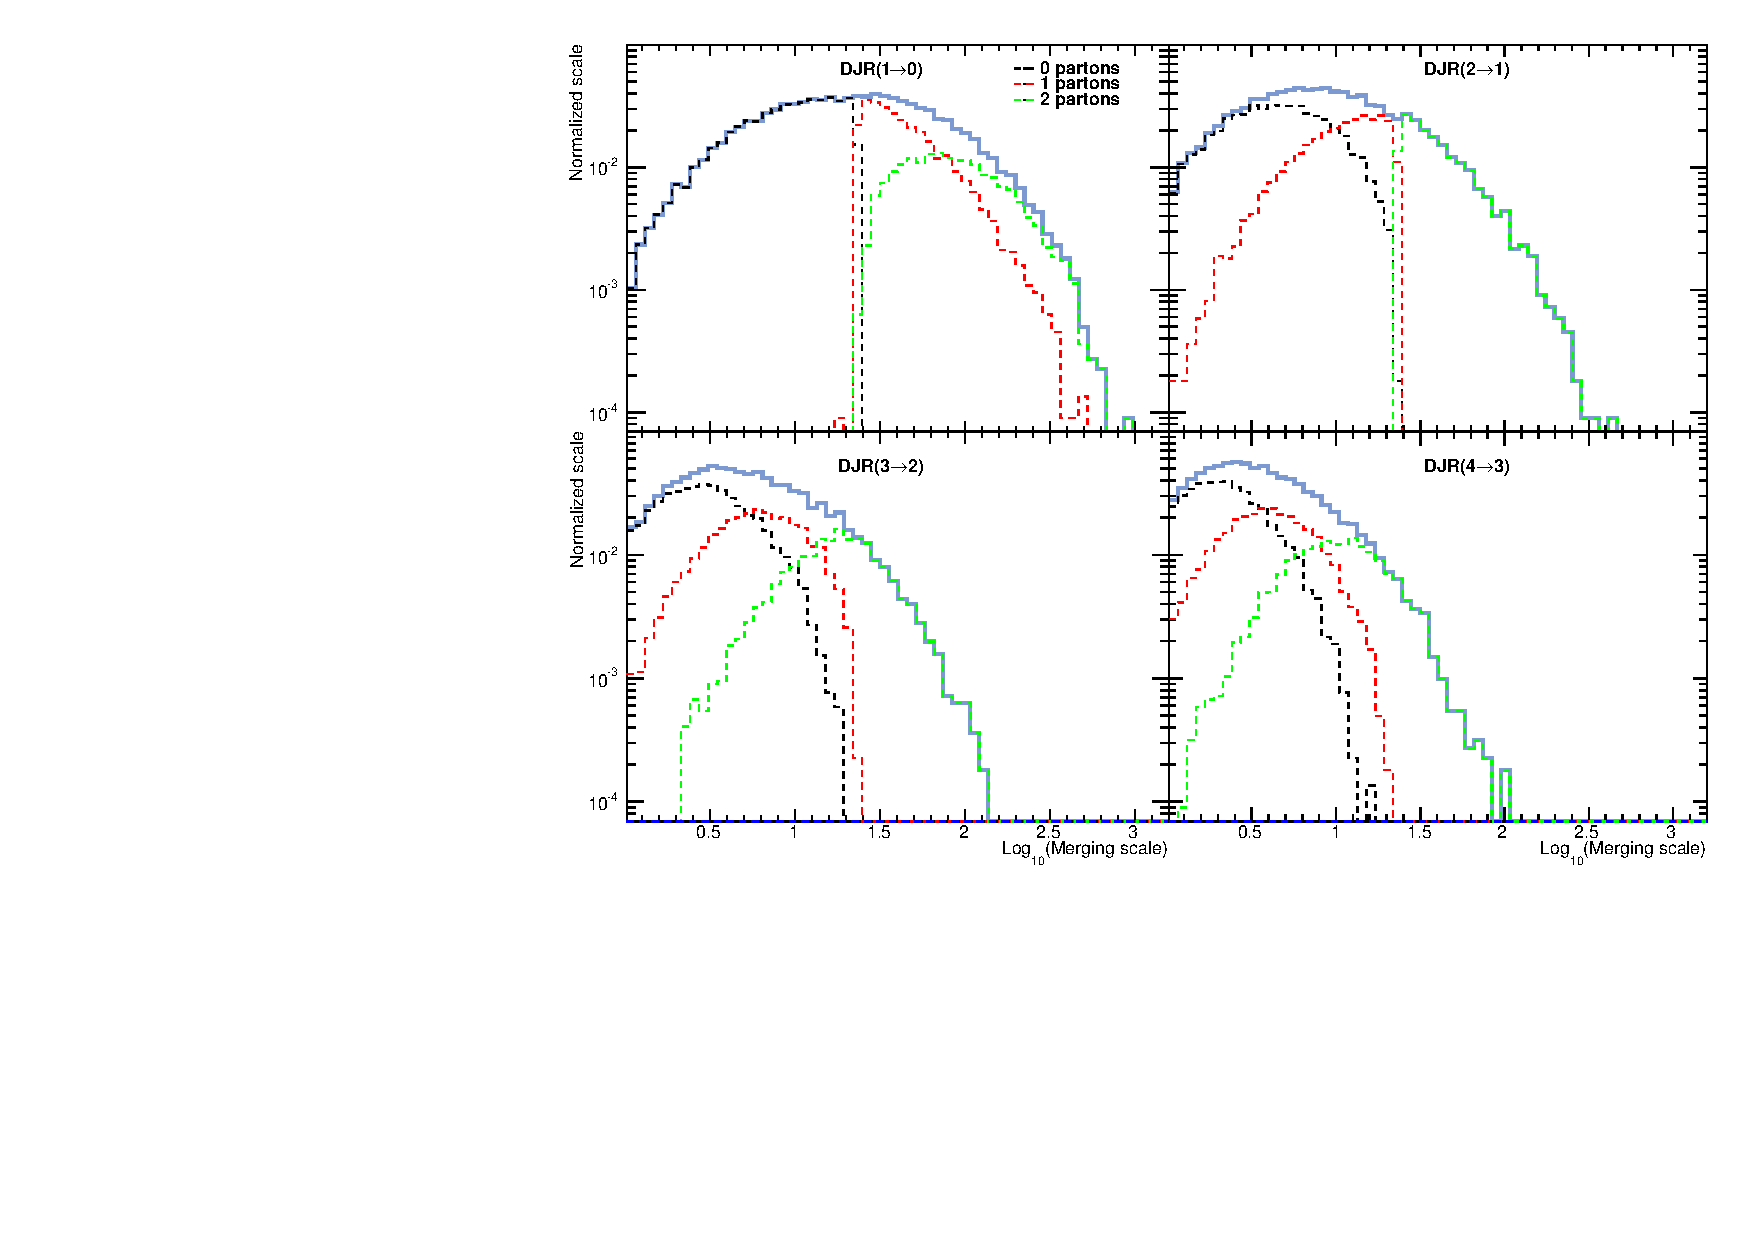
\includegraphics[width=0.80 \linewidth]{figures/WinoNLSP_chargino130_bino1_101_hw_www_DJR.pdf}
\caption{An example of a JDR plot for the Wino NLSP scenario for a top squark mass of $200\,\GeV$ and chargino mass of $150\,\GeV$ for xqcut = 15 and qcut = 23.}
\label{fig:fd_spec_T1}
\end{center}
\end{figure}


\begin{verbatim}
[shell prompt]$ cmsRun 
Hadronizer_MgmMatchTuneZ2star_8TeV_madgraph_tauola_cff_py_GEN.py 
inputFilename="WinoNLSP_chargino130_bino1_101_hw_www.lhe" 
outputFilename="WinoNLSP_chargino130_bino1_101_hw_www.root" 
maximumEvents=-1 qCut=23
[shell prompt]$ root -b -l -n 'plotDJR.C("events.tree",
"WinoNLSP_chargino130_bino1_101_hw_www_DJR.pdf",
"WinoNLSP_chargino130_bino1_101_hw_www.root")'
\end{verbatim} 



%%%%%%%%%%%%% Prospino %%%%%%%%%%%%%%%%%%%%%
\section{\texorpdfstring{$\PROSPINO$}{Prospino}}

\subsection{Introduction}

$\PROSPINO$2 is a computer program which computes next-to-leading order cross sections for the production 
of supersymmetric particles at hadron colliders~\cite{Beenakker:1996ed}. The processes currently included 
are squark, gluino, stop, neutralino/chargino, and slepton pair production. They have also included the associated 
production of squarks with gluinos and of neutralinos/charginos with gluinos or squarks and most recently leptoquark 
pair production. 

The physics results are usually published, so you can cross check the results you get. As far as referencing goes, 
they will not publish a complete Prospino2 manual, because there are physics papers available for all processes. 
Instead, we would like you to reference the published papers for the respective processes. 

There has been a Fortran77 version of Prospino availabe for several years. The increased number of processes 
and the more complex set of input parameters have made it more convenient to migrate to Fortran90. The new 
code should run with any F90 compiler - for example the free gfortran, which even runs on your Macs. 

Prospino2 can easily be linked to C++ programs, reads the Les Houches SUSY spectrum files and includes a set 
of easily accessible interfaces. 

For the third generation $\PROSPINO$2.1. allows you to treat the sbottom and stop channels differently. In this version 
there are also switches to compute the combined renormalization/factorization scale variation and allow for 
non-mass-genenerate light-flavor squarks 
(\url{http://www.thphys.uni-heidelberg.de/~plehn/index.php?show=prospino&visible=tools}).


\subsection{Calculating cross sections}

You will have to download $\PROSPINO$ and untar it.
\begin{verbatim}
[shell prompt]$ tar -xzvf on_the_web_9_23_12.tar.gz 
\end{verbatim}

In order to calculate a cross section for you signal you will have to create a softlink to your SLHA file in 
on\_the\_web\_9\_23\_12 and modify the configuration file.

\begin{verbatim}
[shell prompt]$ ln -sf ln -sf 
../Pythia/slha/coNLSP_chargino1400_gluino1700_delta0.slha 
prospino.in.les_houches
\end{verbatim}

We now configure the $\PROSPINO$ program to calculate gluino-gluino production cross section for 
the slepton co-NLSP scenario. Below is an example of the configuration file.

\lstinputlisting[language=Fortran,linerange={1-106},caption=Example of prospino\_main.f90. $\PROSPINO$ configuration file which will calculate NLO cross sections.]{"links/prospino_main.f90"}

We use inlo=1 to calculate the NLO cross section. Since the squark masses are degenerate in the 
slepton co-NLSP scenario we use the isq\_ng\_in = 0 option. We are interested in physics at the LHC with 
$\sqrt{s} = 8\,\TeV$ so we use icoll\_in = 3. We are also interested in seeing how the NLO cross section varies 
with different factorization scales ($\mu_{f}$) in order to estimate a theory uncertainty though this has not been 
the case in the past. We can calculate the cross section with 0.5$\mu_{\textrm{F}}$ (scale down), $\mu_{\textrm{F}}$ (central), 
and 2$\mu_{\textrm{F}}$ (scale up) by setting i\_error\_in = 1. To calculate the gluino-gluino cross section we 
set final\_state\_in = 'gg'. Since we are not calculating anything with neutralinos/charginos, sleptons, top 
or bottom squarks we set ipart1\_in = 1 and ipart2\_in = 1. Again, we are not doing anything with squarks 
we can set isquark1\_in = 0 and isquark2\_in = 0.

We can now compile and run the program.
\begin{verbatim}
[shell prompt]$ make
[shell prompt]$ ./prospino_2.run >& 
coNLSP_gluino1700_chargino1400_gg.log &
\end{verbatim}

The central value for the gluino-gluino cross sections is in prospino.dat file with a value of 0.454E-04 pb.

We now try to calculate the squark-gluino and squark-squark cross section. To do this we open up 
prospino\_main.f90 and make the following modifications final\_state\_in = 'sg' and we keep ipart1\_in = 1
and  ipart2\_in = 1 the same. We keep isquark1\_in = 0 and isquark2\_in = 0 since we are interested in all 
possible flavors of squarks. Similarly, for squark-squark production we use final\_state\_in = 'ss'. The model 
in which ipart1\_in = 1 and  ipart2\_in = 1 where ever changed was for the natural higgsino NLSP scenario 
which had top squark pair production and neutralino-neutralino pair production. We never ran into a 
scenario in which isquark1\_in = 0 and isquark2\_in = 0 were set to anything other than zero.


%%%%%%%%%%%%% feynMP %%%%%%%%%%%%%%%%%%%%%
\section{Drawing Feynman diagrams with feynMF/feynMP}

\subsection{Introduction}

feynMF (Feyman Metafont) and feyMP (Feynman Metapost) are packages made by Thorsten Ohl to 
draw Feynman diagrams in \LaTeX environment~\cite{Ohl:1995kr}. You can download bundled feynmf.zip from
\url{http://www.ctan.org/tex-archive/macros/latex/contrib/feynmf}.


%%%%%%%%%%%%% feynMP %%%%%%%%%%%%%%%%%%%%%
\section{Summary}

A brief guide has been written that spans a wide variety of MC production tools. In the interest of brevity 
and relevance we have decided against a more comprehensive guide. The softwares documented in this note 
were the ones used most often during these last few years by the Rutgers multilepton group for CMS analyses 
at the LHC during Run \uppercase\expandafter{\romannumeral 1\relax}.


\section{References}

% >> acknowledgements (for journal papers)
% Please include the latest version from https://twiki.cern.ch/twiki/bin/viewauth/CMS/Internal/PubAcknow.
%\section*{Acknowledgements}
% ack-text

%% **DO NOT REMOVE BIBLIOGRAPHY**
\bibliography{auto_generated}   % will be created by the tdr script.

%% examples of appendices. **DO NOT PUT \end{document} at the end
%\clearpage
\appendix
\section{Appendix}

Example of a shell script that produces an SLHA file using $\ISASUSY$.
\lstinputlisting[language=sh,label={lst:HadronicRPV},caption=Example HadronicRPV.sh. Shell script that produces an SLHA file using the $\ISASUSY$ program.]{"links/HadronicRPV.sh"}

Example of a shell script that produces an SLHA file using $\ISASUGRA$.
\lstinputlisting[language=sh,label={lst:mSUGRA},caption=Example mSUGRA.sh. Shell script that produces an SLHA file using the $\ISASUGRA$ program.]{"links/mSUGRA.sh"}

Example of an EDFilter code.
\lstinputlisting[language=sh,label={lst:EDFilter},caption=Example MultiLeptonFilter.cc.]{"links/MultiLeptonFilter.cc"}

%%% DO NOT ADD \end{document}!

